%%%%%%%%%%%%%%%%%%%%%%%%%%%%%%%% 
\section{The Charge Readout System} 
\label{sec:detectors-fd-alt-chg-readout}

In the dual-phase LArTPC concept, the ionization electrons are multiplied in avalanches 
occurring inside detectors, the Large Electron Multipliers (LEMs), located in the argon gas 
phase above the liquid argon level. The drift field of the TPC brings the electrons up to the liquid argon surface where they can  be   
extracted into the gas using a 2-kV/cm electric field defined across the liquid-gas interface.
This extraction field is applied between a submersed extraction
grid (stainless steel wires tensioned in both $x$ and $y$
directions) and the bottom side of the LEMs.
The LEMs are printed circuit boards oriented horizontally, with
conductive layers (electrodes) on the top and bottom surfaces, and many holes drilled
through. The holes form a micro-pattern structure within which the amplification occurs.  
By applying voltages across the two
electrodes of the LEM, a 30-kV/cm electric field region is defined in the holes\cite{Bondar:2008yw}.
Electrons transiting these high electric field regions in the holes trigger Townsend multiplication in the
pure argon gas.


The amplified charge is then collected and recorded on a 2D anode
consisting of two sets of 3.125-mm-pitch gold-plated copper strips that provide the $x$
and $y$ coordinates (and thus two views) of the event.

Typical electric fields between each stage of the readout are
illustrated in Figure~\ref{fig:setup}. Table~\ref{tab:crp_dist} shows
the inter-stage distance and the tolerances required to obtain
uniformity of gain to within $\sim$5\%.
\begin{cdrfigure}[Dual-phase readout]{setup}{Illustration of the electric fields in the amplification region of a dual-phase LArTPC. The simulated field lines in dark blue indicate the paths followed by the drifting charges (without diffusion).}
 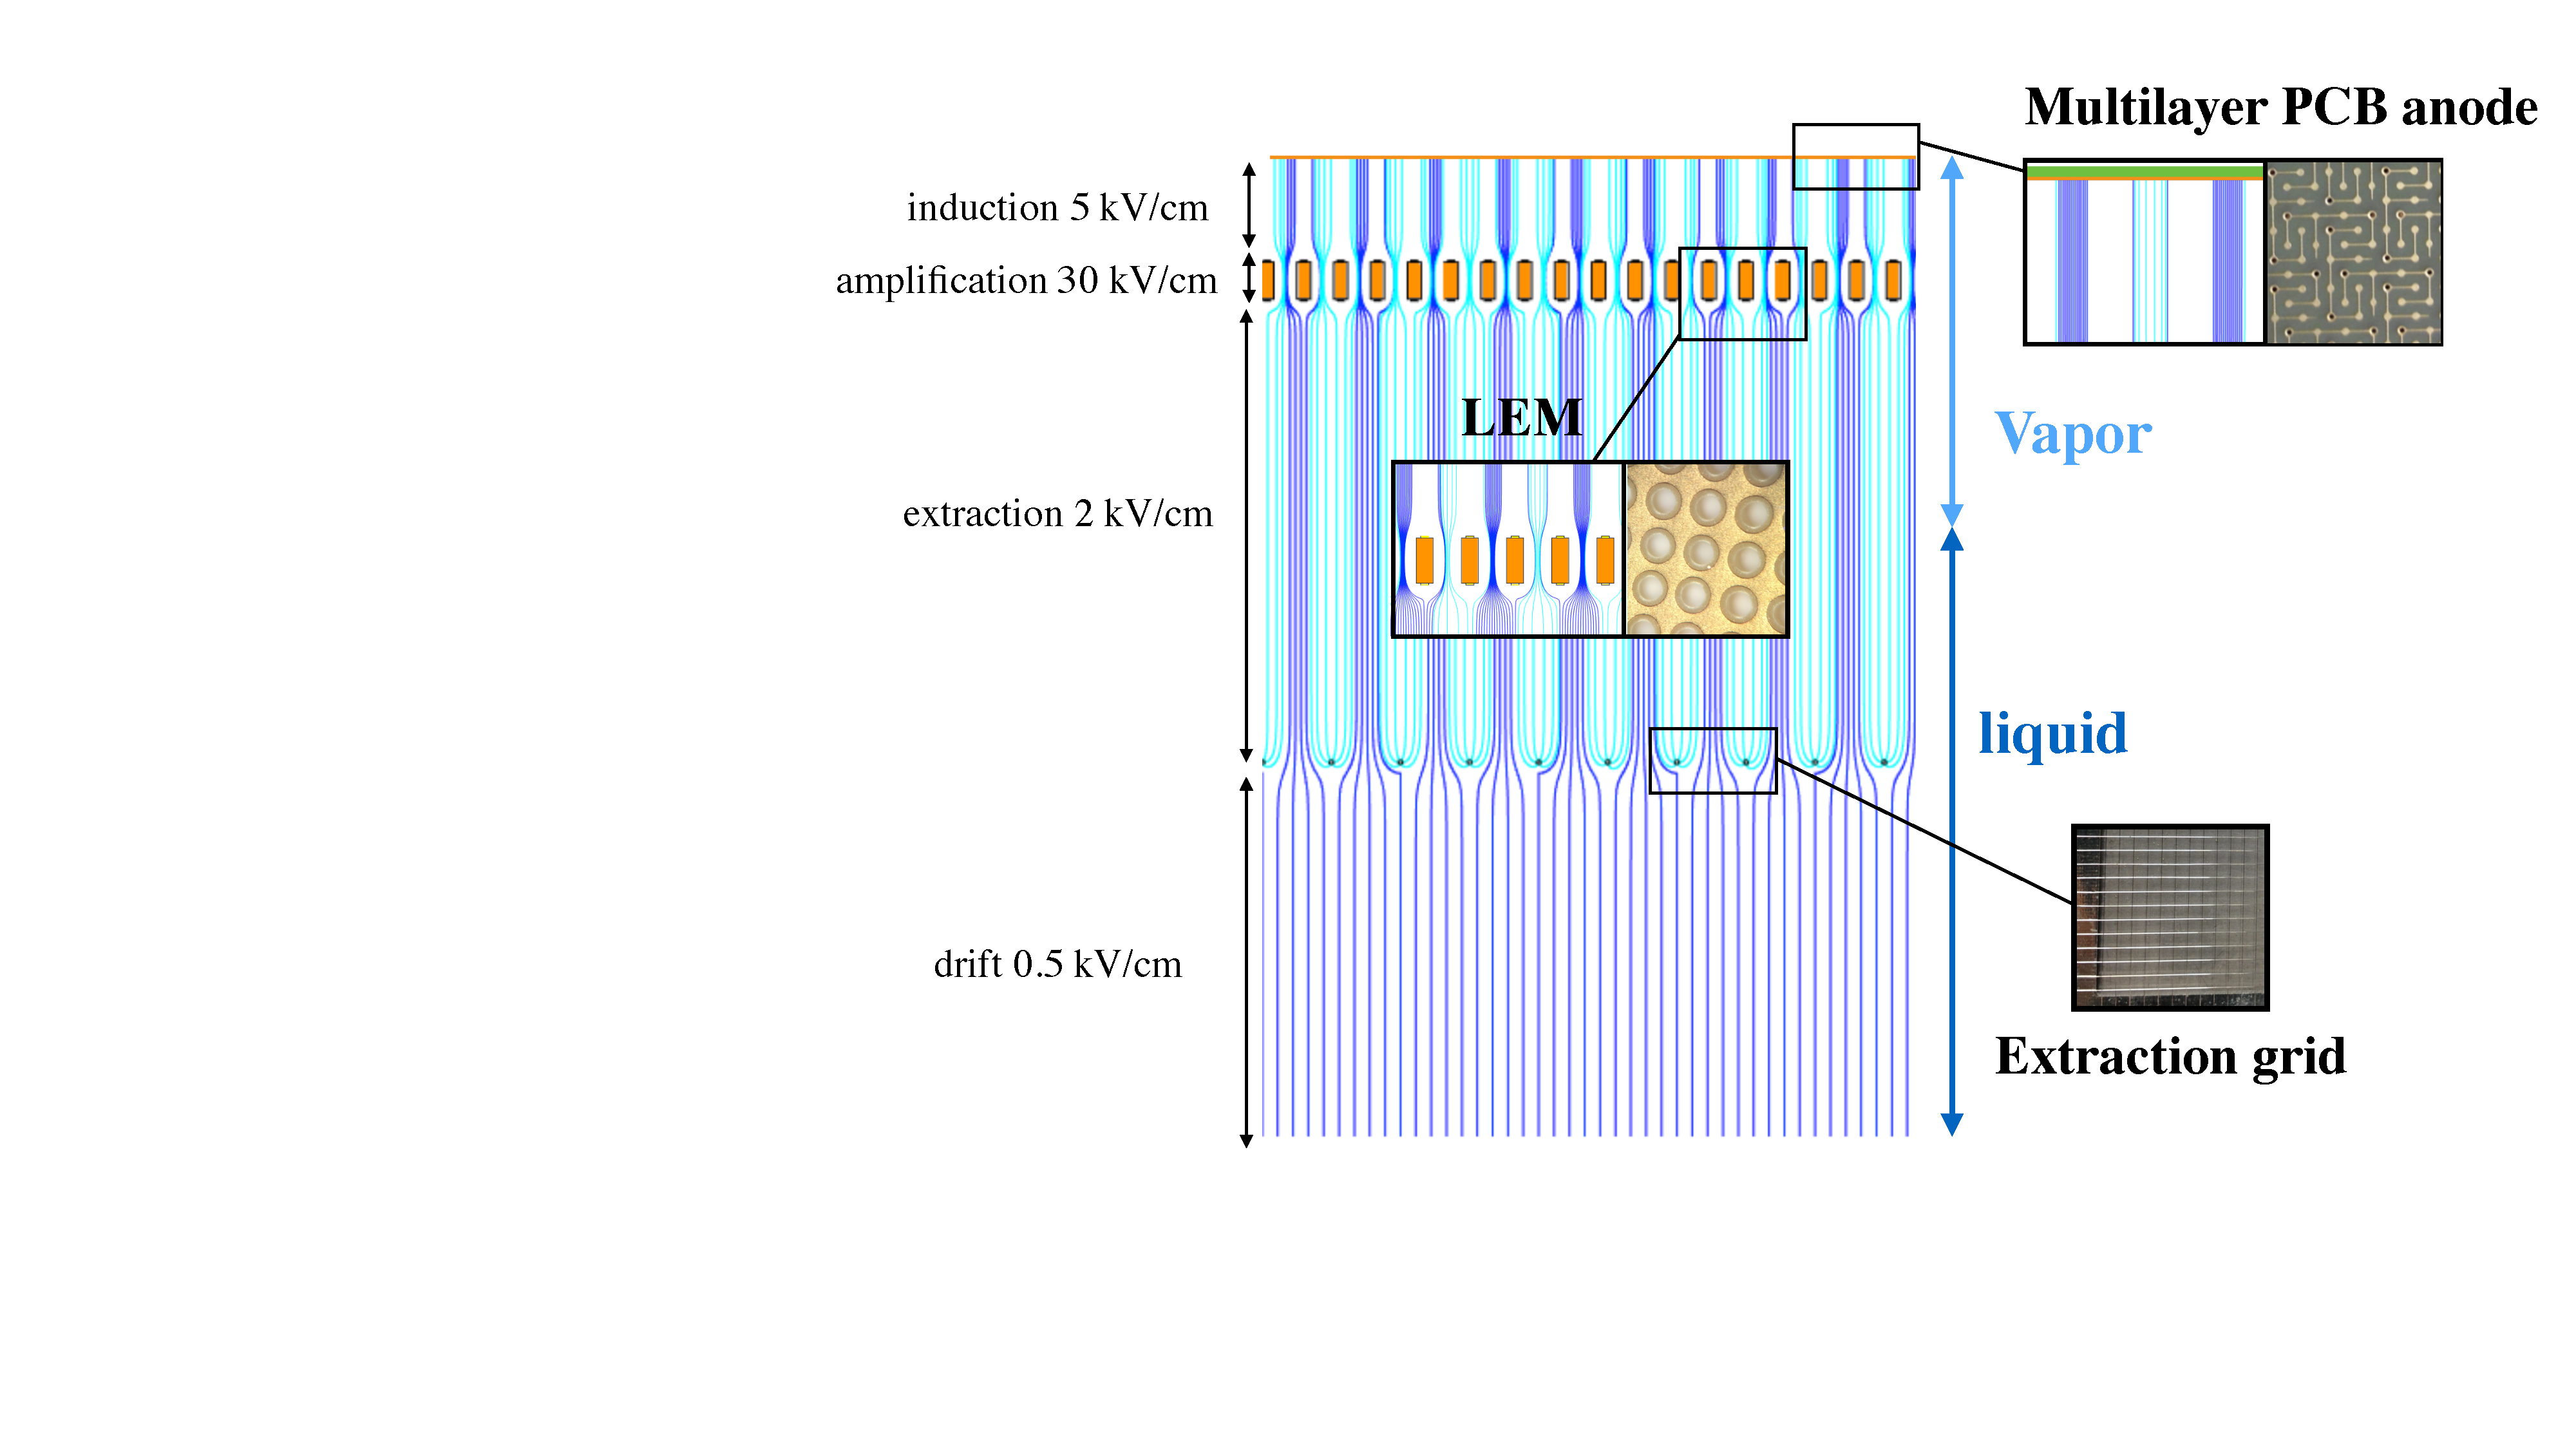
\includegraphics[width=.8\textwidth]{double_phase_principle.pdf}  
\end{cdrfigure}
\begin{cdrtable}[Interstage distances and electric field settings of the dual-phase readout components]{lp{2cm}p{2cm}l}{crp_dist}{Interstage distances and electric field settings of the dual-phase readout components.} 
 Component & Distance [mm] & Tolerance [mm] & Electric field [kV/cm]  \\ \toprowrule
 Anode-LEM top electrode  & 2 & 0.1 & 5\\ \colhline
 LEM top-bottom electrode   & 1 & 0.01 & 30-35\\ \colhline
 LEM bottom electrode-grid        & 10 & 1 & 2 (in LAr) and 3 (in GAr)\\
 \end{cdrtable}

The extraction grid, LEM and anode are assembled into three-layered ``sandwiches'' with precisely defined inter-stage distances and inter-alignment,  which are then connected together horizontally into
modular units of area \num{9}~m$^2$. These units are called Charge Readout Planes (CRPs).


\subsection{The Charge Readout Plane (CRP)}

Each CRP is an independent detector element that performs charge
extraction, multiplication and collection, and has its own high
voltage system and independent signal feedthroughs. The entire area of
the LEM and anode in a CRP is active.

The LEM and corresponding anode are pre-mounted in units of 50$\times$50~cm$^2$, called
LEM/Anode Sandwich (LAS) modules, before being assembled with an extraction
grid into a CRP. Each
anode in a LAS is segmented in 50-cm long $x$ and $y$ strips . Adjacent LAS anodes
are bridged together to form readout strips of the required length by
connecting short flat cables to KEL connectors soldered onto the top
sides of the anodes. The signals from the last anode in each 
strip chain are brought to feedthroughs
mounted on the other side of the front-end electronics embedded inside
dedicated signal-feedthrough chimneys using 50-cm-long flat cables.

The LBNO 20-kt detector design (described in \anxlbnob) featured
modularized CRPs of dimensions of 4$\times$4~m$^2$, with 2-m long
anode strips. For the DUNE cryostat geometry, a size of 3$\times$3~m$^2$
with a strip length of 3~m is found to be optimal. The description in
this section is based on the LBNO 4$\times$4~m$^2$ CRP.

Each CRP is independently hung from the vessel deck through its three
suspension feedthroughs. It has its own high voltage system and 
independent signal and slow-control feedthroughs.
Figure~\ref{fig:4_4CRP_FRONT} illustrates the 4$\times$4 m$^2$ CRP;
its characteristics are summarized in Table~\ref{tab:crp_para}.


\begin{cdrfigure}[Side and top views of the $4\times4$~m$^2$ LBNO CRP]{4_4CRP_FRONT}{Side and top views of the $4\times4$~m$^2$ CRP designed for LBNO (units in mm).}
 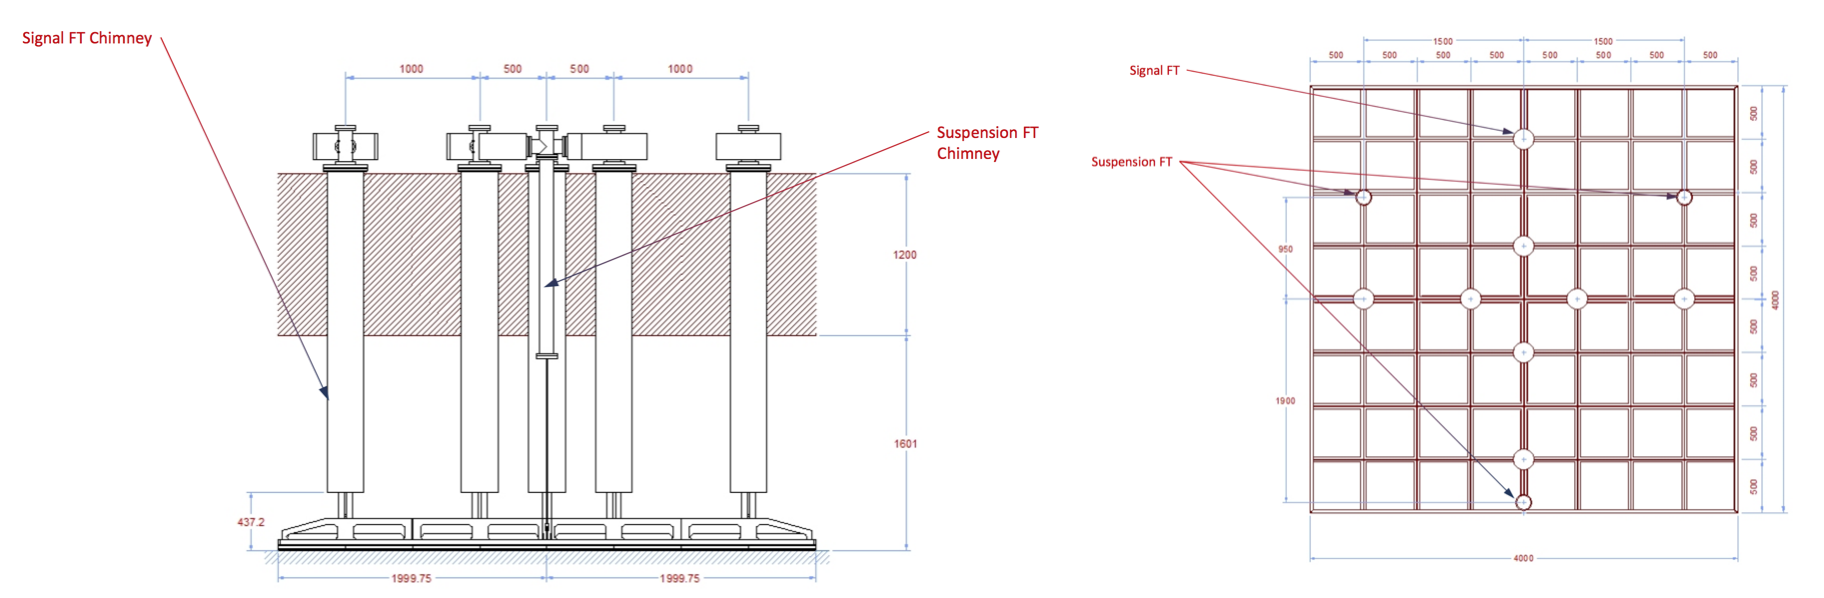
\includegraphics[width=\textwidth]{4_4_CRP_top-side-view}  
\end{cdrfigure}
\begin{cdrtable}[Numbers of components of the 4$\times$4 m$^2$ CRP]{lr}{crp_para}{Numbers of components of the 4$\times$4 m$^2$ CRP designed for LBNO} 
Component & Number \\ \toprowrule
$50\times50$ cm$^2$ anode panels & 64\\ \colhline
$50\times50$ cm$^2$ LEM  panels&  64\\ \colhline
Signal  feedthroughs & 8\\ \colhline
Suspension  feedthroughs & 3\\ \colhline
Readout strip length (m)& 2\\ \colhline
Number of channels & 5120\\
\end{cdrtable}

The entire area of the LEM and anode is active, as noted earlier, and
each adjacent 50$\times$50~cm$^2$ LAS module has a gap of only 0.5~mm.
Therefore, the 4$\times$4~m$^2$ area of the CRP is fully 
active; the 0.5-mm edge gaps occurring every 50~cm
do not interfere with the
charge collection in the  
anode, given its readout pitch of 3.125~mm.

The extraction grid consists of 100~$\mu$m diameter stainless steel
wires tensioned in both $x$ and $y$ directions over the entire 4-m
length/width of the CRP  with 3.125~mm
pitch. They are soldered into groups of 32 on independent
wire-tensioning pads oriented perpendicularly to the side of the CRP
frame.  Each wire-tensioning pad consists of a printed circuit board
(PCB) for HV-connection that is fixed very precisely to a mechanical 
wire holder. The PCB has 32 soldering pads with 200-$\mu$m grooves for
precise positioning of the wires. During the wire-soldering process
each wire is tensioned by 150-g lead weights and positioned in a
groove.  (With this method better than 50~$\mu$m precision on the wire
pitch, measured under the microscope, was achieved for the LBNO-WA105
prototypes.) The PCB is then mounted on the wire holder and the
tension of the group of 32 wires can be precisely adjusted by pushing
the holder against the CRP's FR4 frame with two screws.

The wires, $\sim$3~m long in both $x$ and $y$ directions,
have their sags minimized to $\sim$0.1~mm thanks to $x$ and $y$ oriented
supporting comb-teeth blades (see Figure~\ref{fig:Wires_comb}) inserted
between anode planes of 1~m$\times$1~m size. The array of blades
penetrates the liquid surface and has the additional
benefit of maintaining the liquid level still. 

\begin{cdrfigure}[Comb for hanging extraction grid wires]{Wires_comb}{Comb for hanging extraction grid wires}
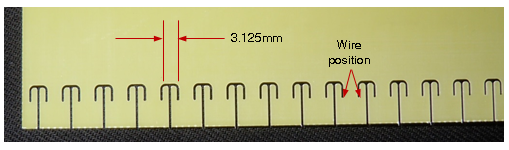
\includegraphics[width=.6\linewidth]{Wires_comb.png}
\end{cdrfigure}

The 4$\times$4~m$^2$ CRP has 5120 readout channels in total. The
signals from the CRP are read out through eight signal feedthroughs
(SFTs) chimneys
at the bottom of which the front-end electronics cards are mounted. Amplified signals
are transmitted to the DAQ system located on top, outside of the vessel.
Each chimney groups 640 channels. 

The 3$\times$3~m$^2$ DUNE CRP, is a down-sized version of the LBNO
CRP; it has three signal feedthrough chimneys and 1920 readout
channels.

Three suspension
feedthroughs are arranged as an equilateral triangle whose barycenter
coincides with that of the CRP; they suspend the CRP at the required
position and precisely adjust the CRP level with respect to the liquid
argon surface. Figure~\ref{fig:4_4CRP_3D} shows a 3D view of the CRP,
where the signal chimneys  (discussed in 
Section~\ref{sec:detectors-fd-alt-elec}) and the stiffening frame are
visible.
\begin{cdrfigure}[3D view of the $4\times4$~m$^2$ CRP.]{4_4CRP_3D}{3D view of the $4\times4$~m$^2$ LBNO CRP.}
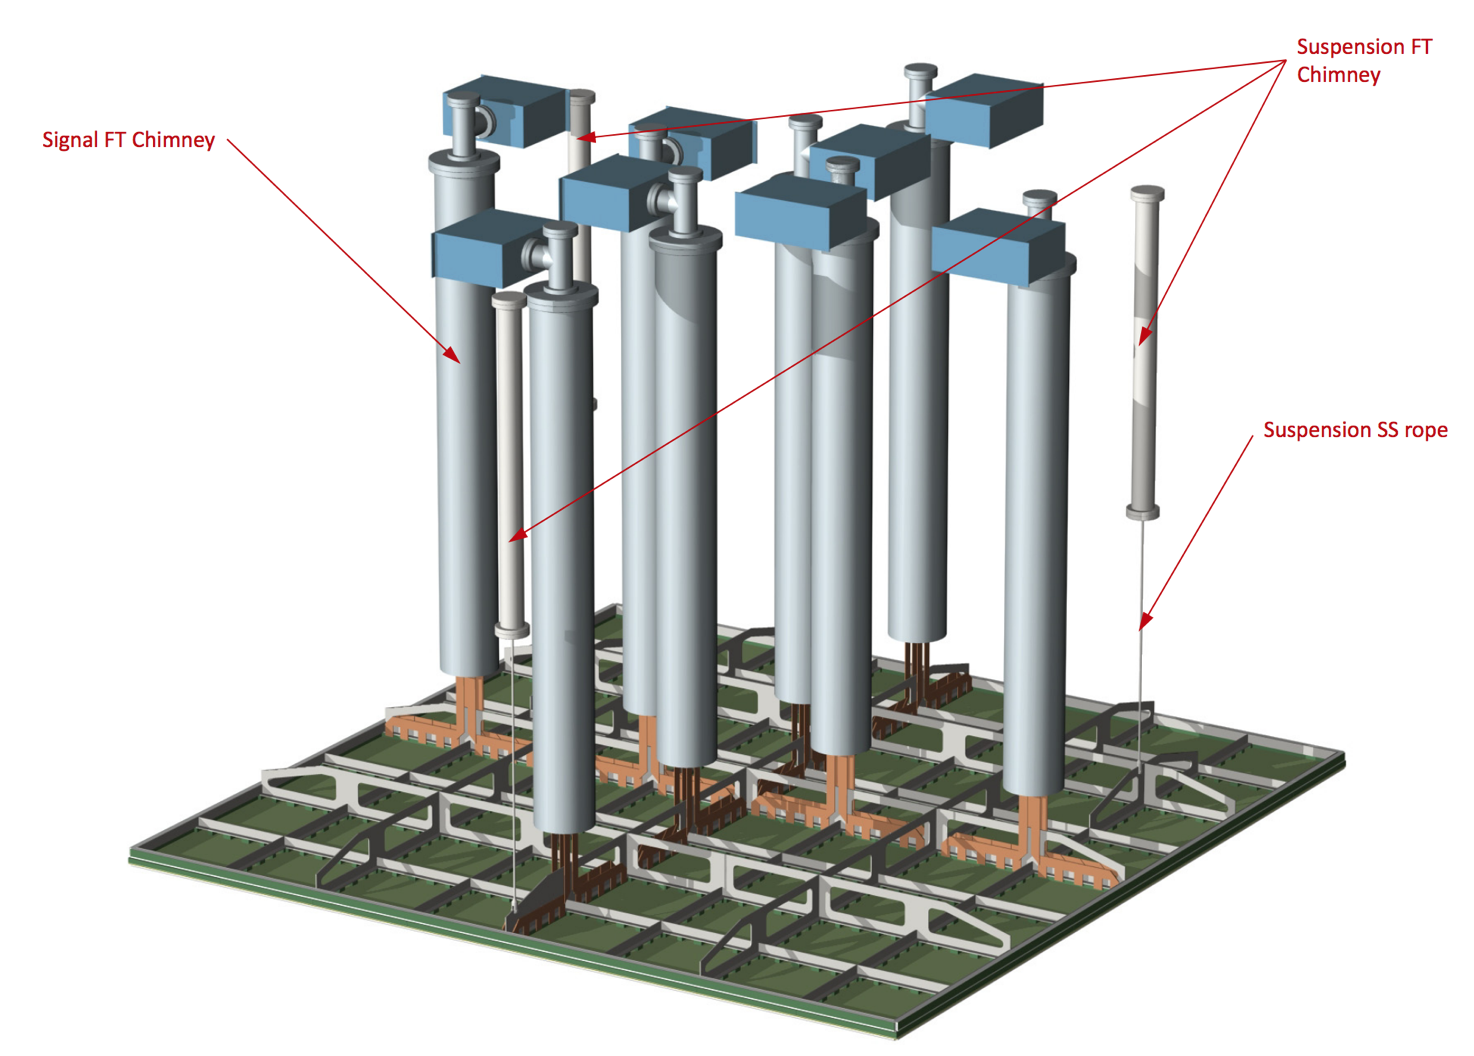
\includegraphics[width=0.8\textwidth]{4_4CRP_3D}  
\end{cdrfigure}


\subsection{The LEM/Anode Sandwich (LAS)}

LAS modules, the CRP building blocks composed of 50$\times$50-cm$^2$ LEM-anode 
sandwiches,  have been extensively studied as part of the ongoing CERN
WA105 prototyping efforts (see~\ref{sec:proto-cern-double}). The LEMs
and the anodes are produced by a PCB manufacturing company called
ELTOS\footnote{\url{www.eltos.it}}. Their designs are the outcome of
intensive R\&D effort over the last few years, aimed at maximizing the
S/N ratio for the large-area readouts envisioned for use in giant
dual-phase LArTPCs.  Figure~\ref{fig:LEM_anode} shows the LEMs and
anodes.  This section summarizes key features of the LAS.


\begin{cdrfigure}[Pictures of the LEM and anode along with microscope views]
{LEM_anode}{Top: pictures of the LEM and anode along with microscope
  views. Bottom: close up of the LEM HV connectors and back view of the anode 
with the KEL signal connectors to bridge to the adjacent LAS or to connect 
flat cables going to the signal feedthrough}
 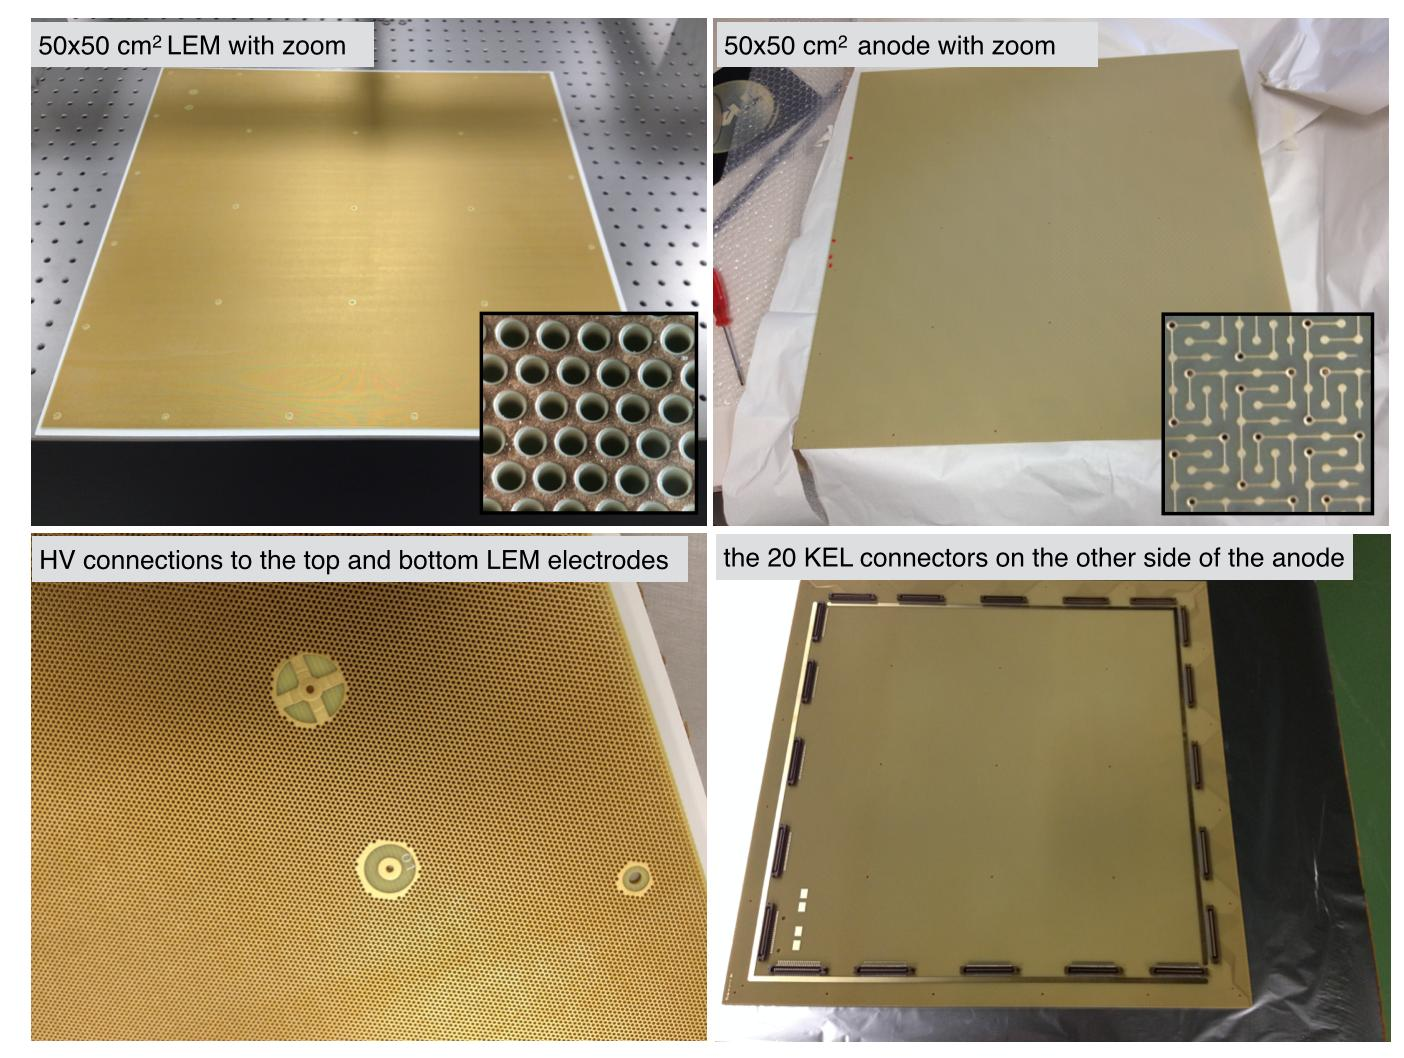
\includegraphics[width=.8\textwidth]{LEM_anode_zoom.jpg}  
 \end{cdrfigure}


 \paragraph{The 50$\times$50~cm$^2$ anode:}

Each  50$\times$50~cm$^2$ anode is manufactured from a single multilayer Printed Circuit
Board (PCB). The readout strips for both $x$ and $y$ views consist of a pattern of
gold-plated copper tracks 
with a 3.125-mm readout pitch. The two views have superimposed track patterns
that are  electrically insulated from one another. Electrical insulation in the points where
the $x$ and $y$ tracks would superimpose is achieved by having tracks crossing
over and under each other using a system of vias between the top and bottom layers of the PCB.
 
The design of the track patterns forming the strips is such that both $x$ and $y$ views
collect the same amount of charge, independent of the angle of
charged-particle tracks with respect to the readout strip
orientation. The tracks pattern should then ensure a uniform and isotropic coverage of the strip surface while 
minimizing the strip capacitance. These criteria have driven a thorough design optimization.  
Various PCB layouts were tested in order the achieve the best performance, as described in~\cite{Cantini:2013yba}. 
The final layout and schematic of the anode are shown in Figure~\ref{fig:anode_sch}. 

\begin{cdrfigure}[The 2D anode]{anode_sch}
{The 2D anode (left) and its schematic showing the  interconnections  ensuring continuity within each view while preserving insulation
with respect to the perpendicular view  (right). One view is filled  in red and the other in white.}
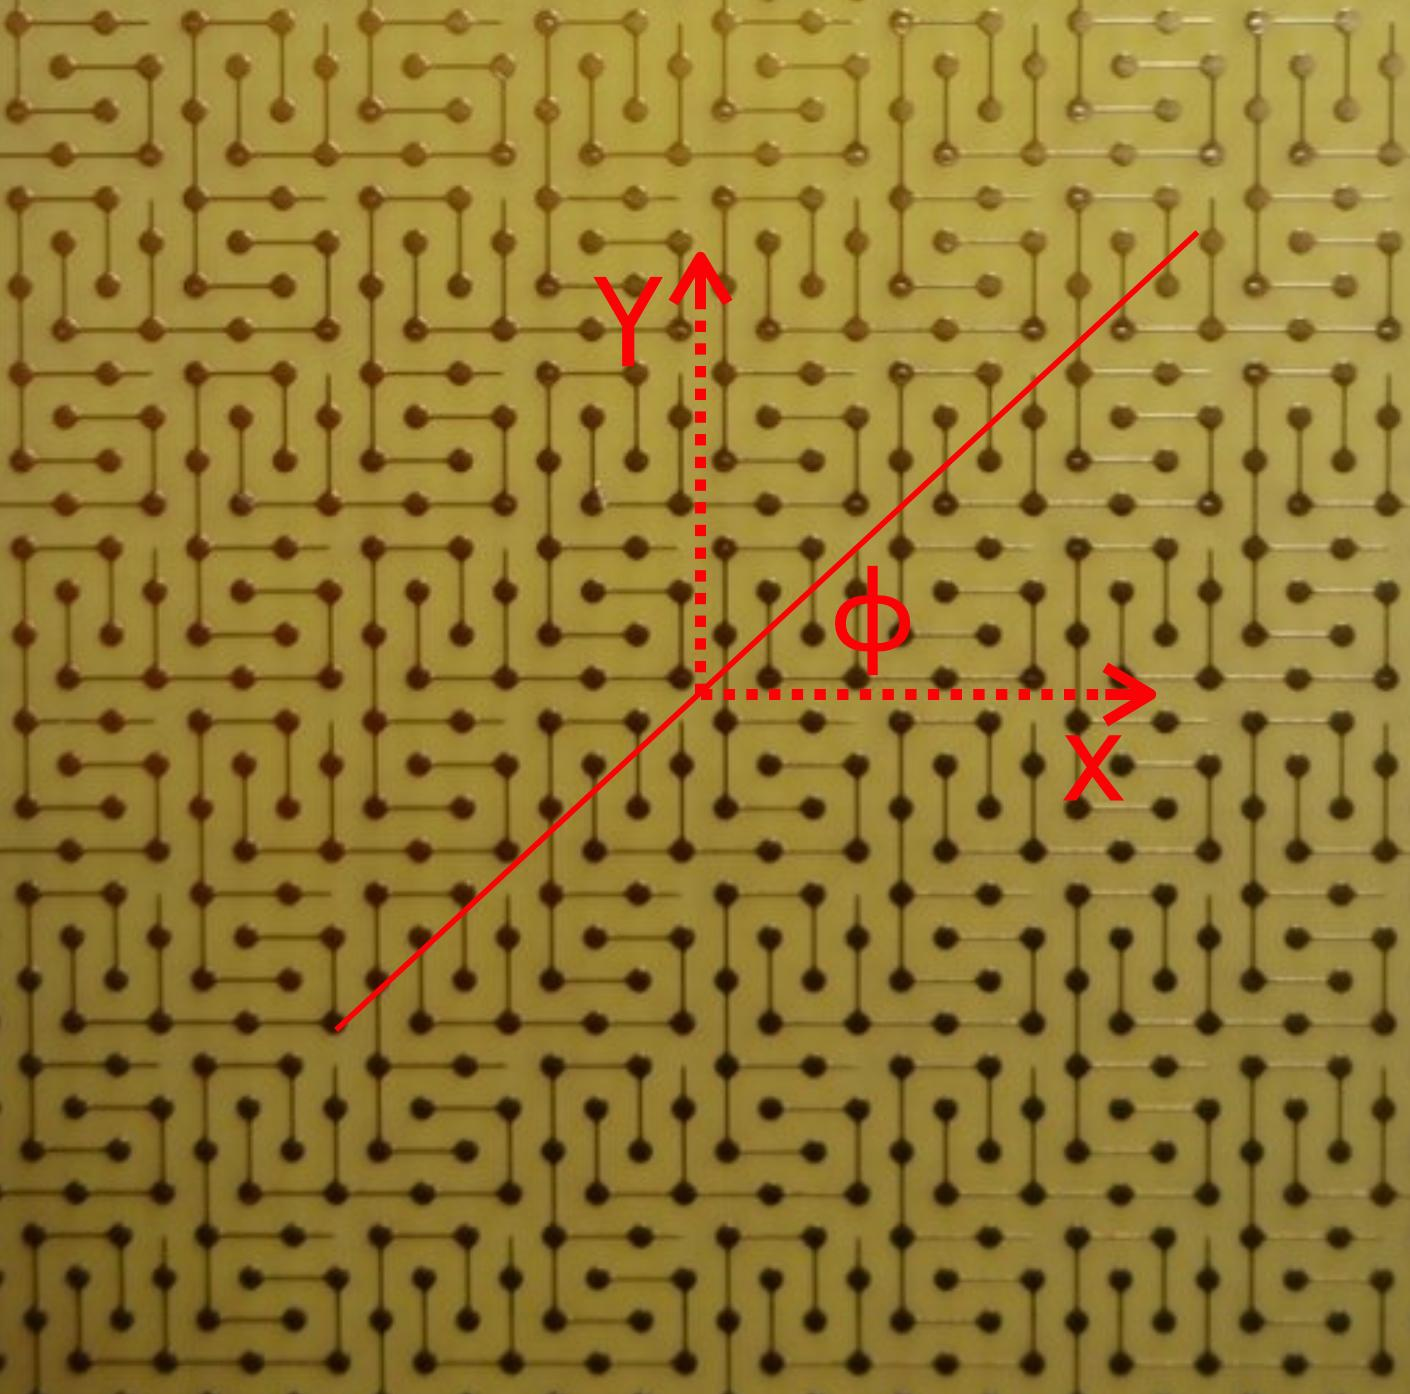
\includegraphics[scale=0.2]{anode_pcb.jpg} \hspace{0.2cm} 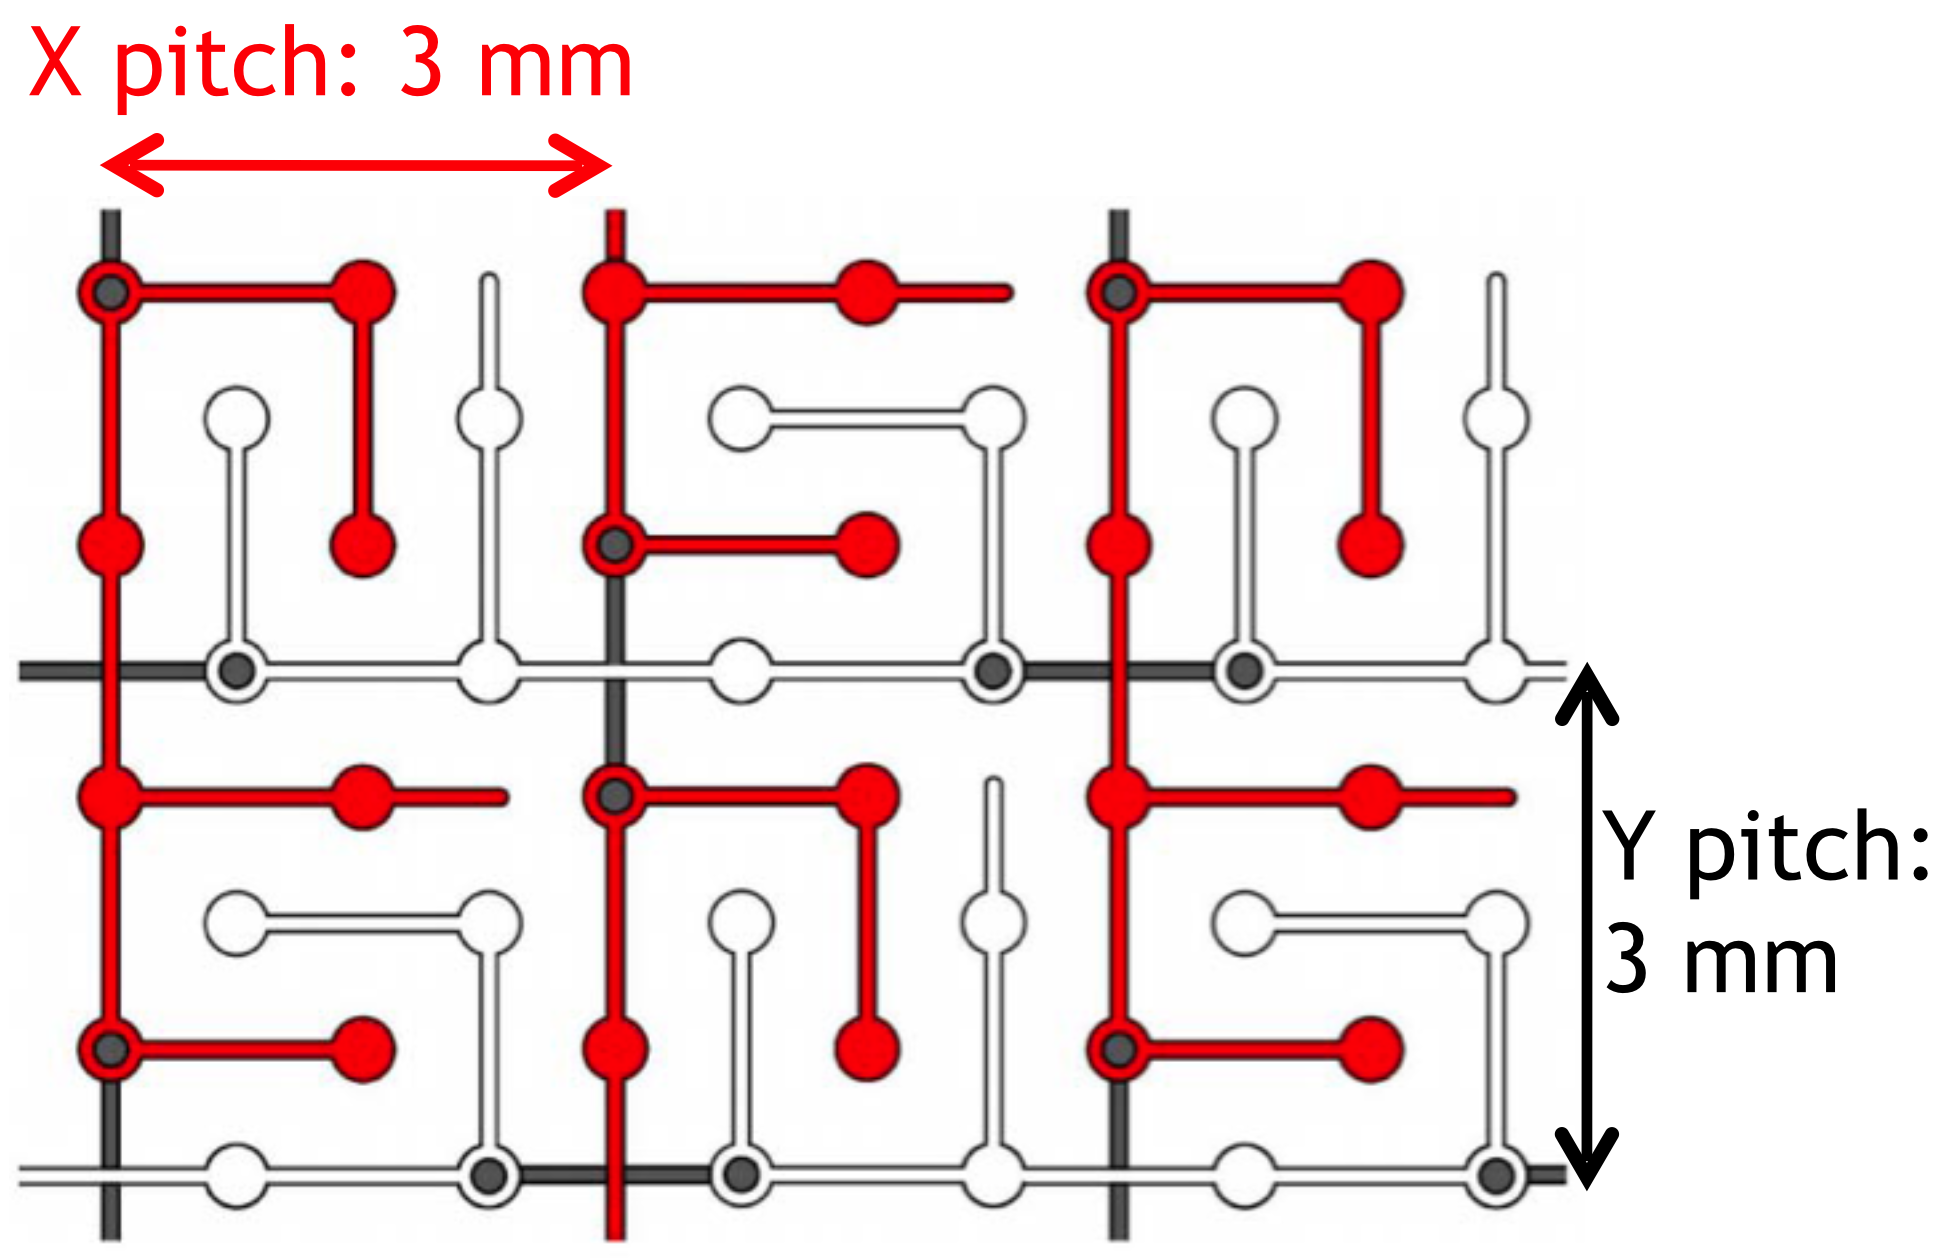
\includegraphics[scale=0.2]{anode_sch}
\end{cdrfigure}

As result of this optimization, the electrical capacitance of the
readout strips has been limited to only 150~pF/m, which translates
into an electronic noise of about $\sim$1000 electrons for a 2-m readout
length.  Figure~\ref{fig:anode_res} (right) shows that the
charge-sharing asymmetry between the two views is kept within 1\%. 
The two views can thus be treated in a completely equivalent way
from the point of view of the reconstruction. The response in terms of
the charge collection per unit pathlength $\Delta Q/\Delta s$ is
independent of the charged-particle tracks' azimuthal angle $\phi$
(see Figure~\ref{fig:anode_res} left and middle).
\begin{cdrfigure}[Charge deposition as function of track angle ]{anode_res} {Charge deposition per unit of pathlength measured on LEM view 0 
($\Delta Q_0/\Delta s_0$) as a function  of the track angle $\phi$ (left) and  projection of the  $\Delta Q_0/\Delta s_0$ distribution in three $\phi$ intervals (middle).  The right plot  shows the distribution of the difference between the total charge  collected on both views normalized to their sum}
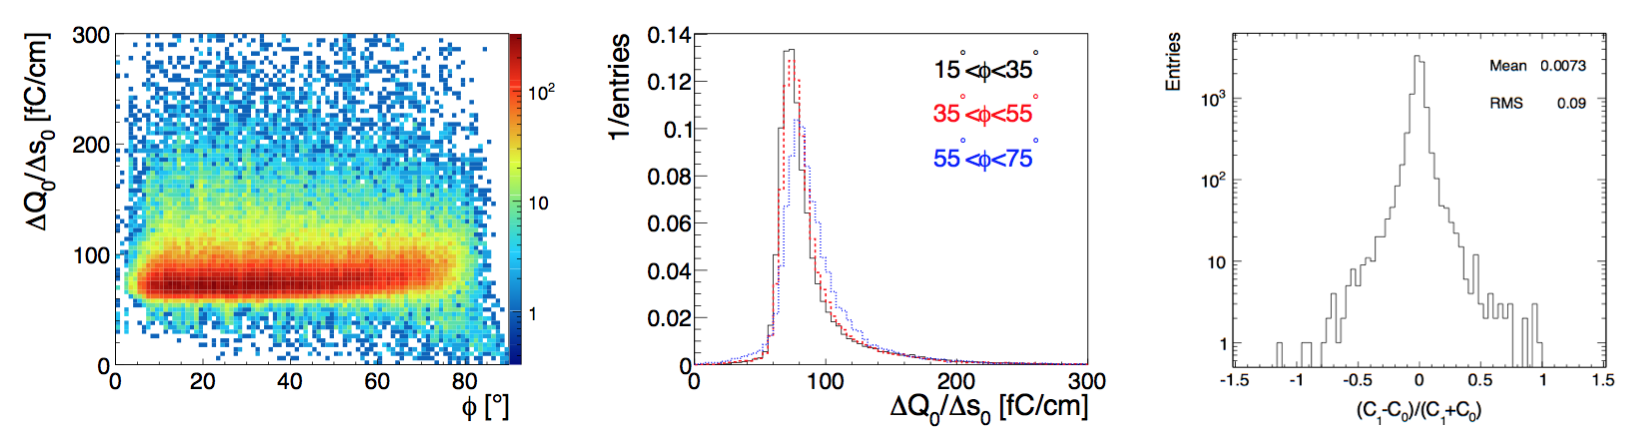
\includegraphics[width=.9\textwidth,scale=1]{anodeD_prop}
\end{cdrfigure}

\paragraph{The 50$\times$50~cm$^2$ LEM:}

Each LEM is built from a 1-mm-thick copper-clad epoxy PCB with
500~$\mu$m diameter holes drilled through, surrounded by a
40-$\mu$m dielectric rim. The holes are arranged in a honeycomb
pattern with a pitch of 800~$\mu$m, resulting in about 200 holes per
cm$^2$ and $\cal O$(500,000) holes over the entire 50$\times$50~cm$^2$
area. The holes provide confinement for the UV photons produced during
the avalanche process and thus act as a mechanical quencher to prevent
photon feedback. This property makes the LEM suitable for operation in
ultra-pure argon vapor without the addition of a quenching gas. 

The amplification of the drifting charges in pure argon vapor at 87~K with
LEMs has been extensively demonstrated on a chamber with
10$\times$10~cm$^2$ area readout (see e.g.,
\cite{Badertscher:2008rf,Badertscher:2010fi}) as well as on
a larger device consisting of a 40$\times$80~cm$^2$
readout\cite{Badertscher:2013wm}.  Both setups were successfully and
stably operated at constant gains of at least 15, corresponding to
S/N $\approx$ 60 for MIPs. Recent studies\cite{Cantini:2014xza}
systematically characterize the impact of the rim size, insulator
thickness, hole diameter and hole layout on 10$\times$10~cm$^2$ area
LEMs. The response in terms of maximal reachable gain and influence on
the collected charge uniformity, as well as the long-term stability of
the gain, has been thoroughly compared for these different
layouts. Some results are shown in Figure~\ref{fig:LEM}.  Gains of
almost 200 were reached and the LEMs could be operated at stable gains
of at least $\sim$15 after a charging up period of about a day.
\begin{cdrfigure}[LEM performance vs geometry]{LEM}{Performance of the LEMs with different geometry parameters. Left: effective gain vs. LEM electric field; right: the stabilizations of the effective gain over time.}
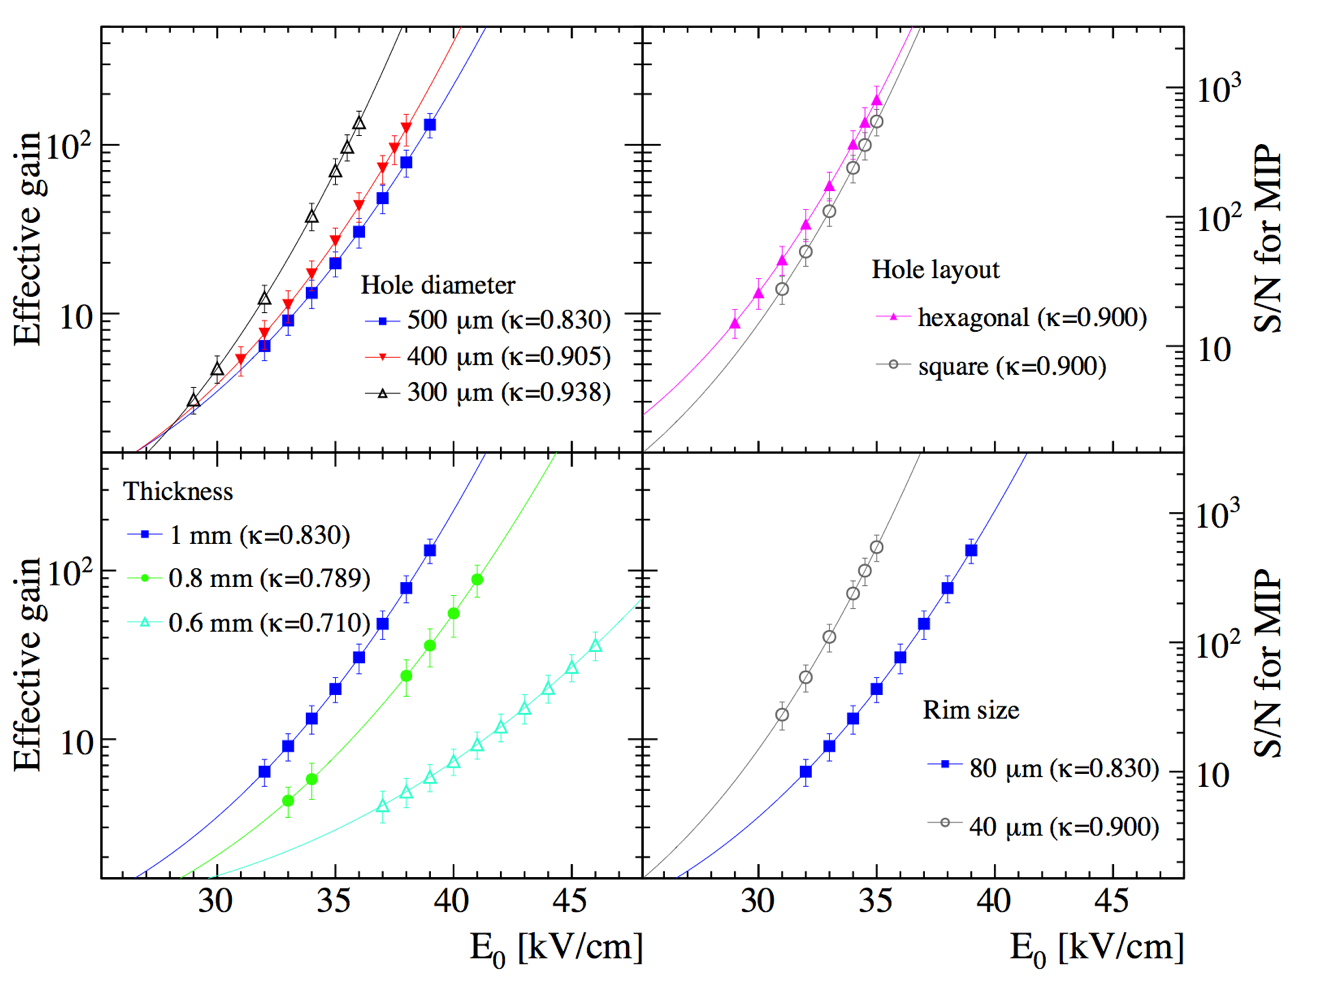
\includegraphics[scale=0.35]{4}
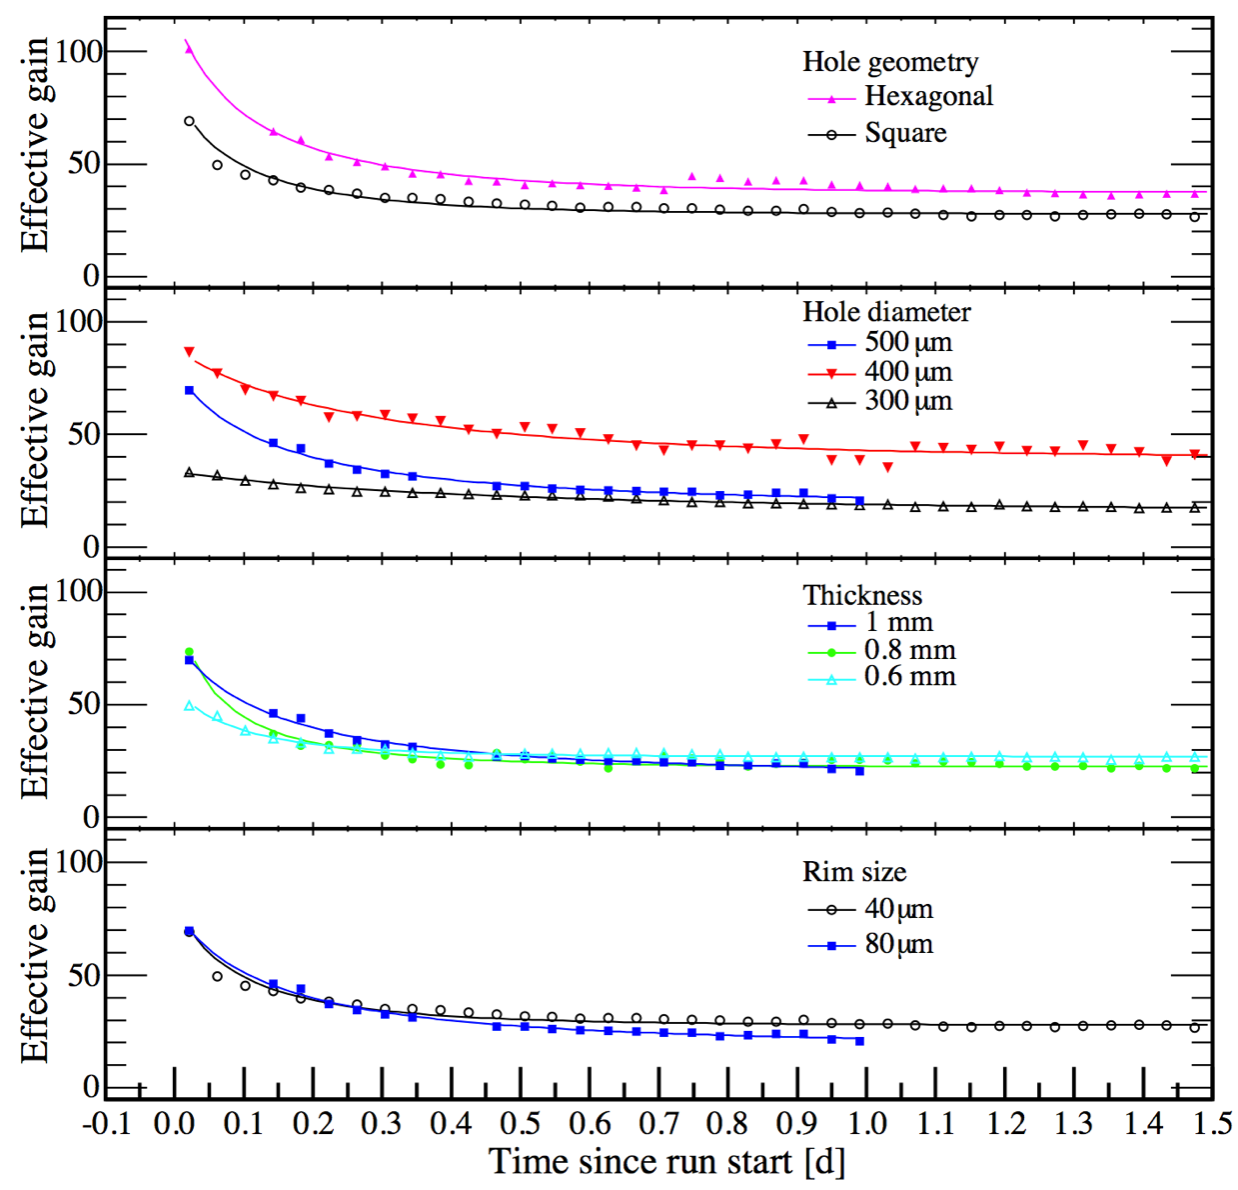
\includegraphics[scale=0.32]{3}
\end{cdrfigure}


\paragraph{LAS Assembly:}

Figure~\ref{fig:LEM_metro} shows the LEM/anode sandwich (LAS).  A LAS is 
fixed together with 29 M2 PEEK screws, each containing a precisely
machined 2-mm-thick pillar to guarantee a constant inter-stage
distance between LEM and anode on the entire $50\times50$~cm$^2$
area.  The dead zones caused by the supporting pillars and the two HV
pins on the LEMs are minimized and make up less than 0.5\% of the
total area. The inter-stage distance between the LEM and anode in the
LAS has been measured at many points. The results are shown in
Figure~\ref{fig:LEM_metro} and are described
in~\cite{EDMS_metro_lem_anode}. They indicate that the planarity is
within the required tolerance of 2~mm $\pm$ 100~$\mu$m .
\begin{cdrfigure}[LEM/anode sandwich metrology]{LEM_metro}{Close up pictures of the LEM/anode sandwich. The two
       bottom figures show a the measurement at the CERN metrology lab
       and a histogram illustrating the measured gap between the LEM
       and anode in various points. As can be seen the distribution is
       centered on the nominal distance of 2~mm and has an RMS of
       about 100$\mu$m.}
     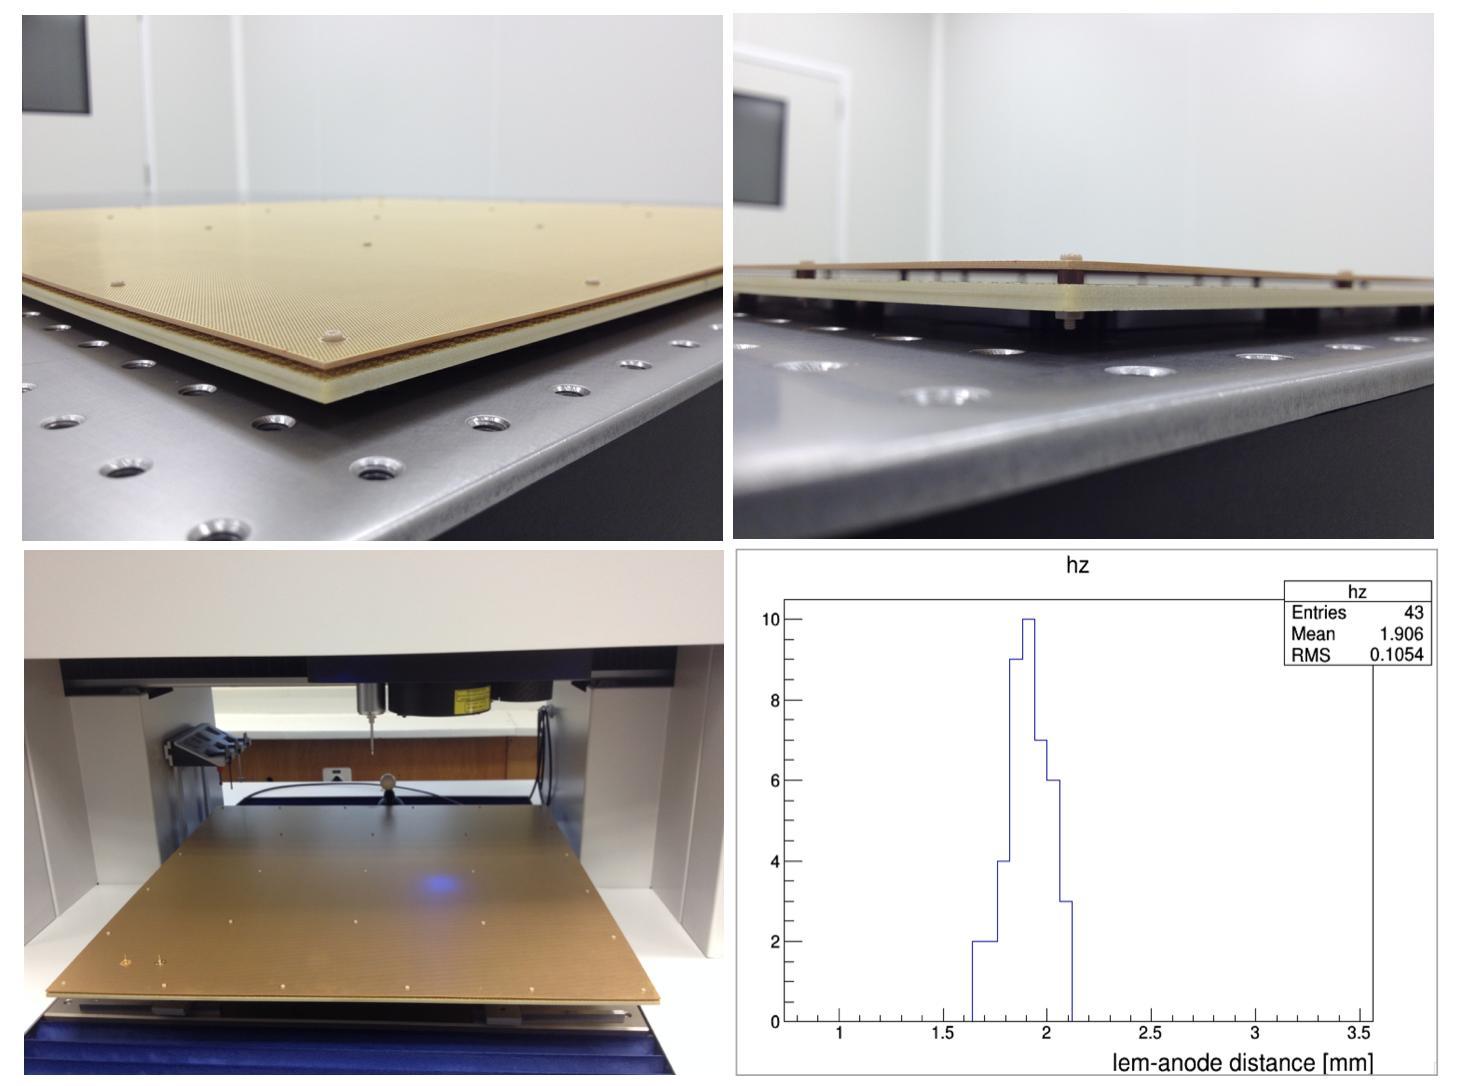
\includegraphics[width=.7\textwidth]{LEM_metro.jpg}
\end{cdrfigure}

The entire mounting sequence of the sandwich as well as that of the
different elements of the CRP are being addressed in the WA105
prototype detectors. An example of a sandwich assembly on a
3 $\times$ 1~m$^2$ CRP is shown in Figure~\ref{fig:CRP_assembly}.
\begin{cdrfigure}[Pictures of the assembly of a $3\times1$m$^2$ CRP]{CRP_assembly}{Pictures of the assembly of a $3\times1$m$^2$ CRP}
     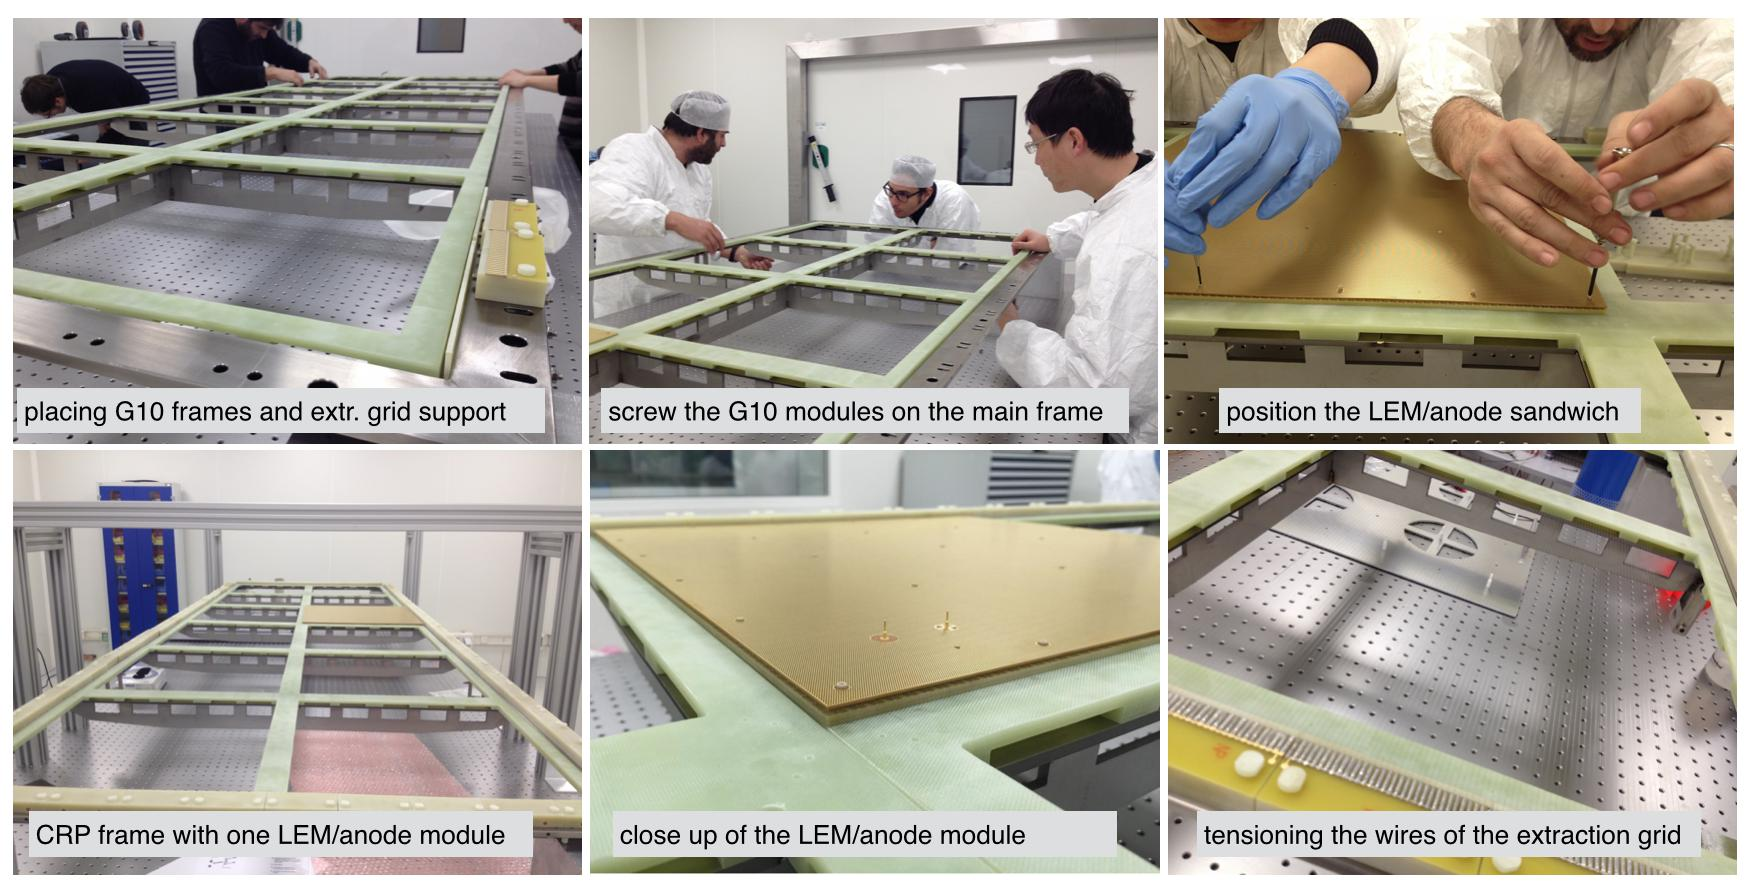
\includegraphics[width=\textwidth]{311_CRP_assembly.jpg}  
\end{cdrfigure}


